\documentclass[a4paper,10pt]{scrartcl}
\usepackage{ngerman}
\usepackage{amsmath, amsfonts, epsfig, xspace}
%\usepackage[LGRx,T1]{fontenc}
\usepackage[utf8x]{inputenc}
\usepackage[greek,english]{babel}
\usepackage{algorithm,algorithmic}
\usepackage[normal,tight,center]{subfigure}
\setlength{\subfigcapskip}{-.5em}
\usepackage{color}

\usepackage{natbib} %für schönere Zitate
\definecolor{Red}{RGB}{255,0,0}
\definecolor{Blue}{RGB}{0,0,255}

\usepackage[colorinlistoftodos,textsize=tiny]{todonotes}

\presetkeys{todonotes}{fancyline}{}

\definecolor{todored}{rgb}{1, 0.6, 0.6}
\definecolor{todoorange}{rgb}{1, 0.8, 0.4}
\definecolor{todoblue}{rgb}{0.4, 0.8, 1.0}
\definecolor{todogreen}{rgb}{0.8, 1.0, 0.4}
\definecolor{todopurple}{RGB}{255, 100, 127}


\newcommand{\comment}[1]{
\todo[bordercolor=todoorange!80!black,color=todoorange]{\textbf{Comment:} #1}
}


%\newcommand{\textgreek}[1]{\begingroup\fontencoding{LGR}\selectfont#1\endgroup}

\newcommand{\cn}{$^\text{[citation needed] }$}

\author{Jonathan Oberländer}

\title{Automatic Detection of Linguistic Quality Violations}

\begin{document}

\maketitle
%TODO
%erst noch sagen, was du genau annotiert hast: die Instanzen, die Marina als ungrammatical_sent markiert hat oder? <tat ich doch, oder?


% 1. corpus analysment
% erste Tests nicht erwähnen<done
% "first step was to inspect the corpus" "other_ungr_forms"<done
% für alle Subtypen ein Beispiel <done
% Namen geben <done
% restrukturieren: incomplete-sentence untertyp von other_ungrammaticality <done
% im Bild Achsen beschriften <done

% 2. method
% was tat ich? "Python" nicht erwähnen (keine technical details)<semidone
% woher kommen die clauses <done
% wie ist der Overlap <???
% allen methoden klaren Namen geben <"done"

%>words that start with a capital letter and are only followed by lower case letters are seen as known words / named entities. <done
% <we assume that .... are also known token <done

% subset von gigaword genau benennen <done

% 3. evaluation
% Tabellen <done
% alles einzeln
% worauf beziehen sich die Zahlen?? <KEINE AHNUNG I AM STUPID
% grafik auf dev-2 notiert (oder beides) < NOCH NICHT GETAN!!!

% auf allen ungrammatical testen //MINDESTENS <done. puh.
% was ist mit den false negatives? <done
	% on subtype:	tagged as other type
	% on all:		actually other ungrammaticality
% Beispiele an Anne schicken

% 4. discussion
% incmpl annotieren mit subtypen
% beobachtung hinschreiben, dass clauses annotiert werden, die incmplsent sind
% evtl. positiv getaggte angucken und 

\section{Corpus Analysis}
%intro foo %TODO

The first step is to inspect the corpus. It is soon noticeable that the type system of the LQVCorpus~\citep{valeeva} isn't detailed enough for our purposes and has a few shortcomings: Especially under the label of \texttt{other\_ungrammatical\_form} many different types of errors are combined. For this reason, we define a number of subtypes for this violation:

\begin{description}
\item[missing spaces] \comment{rename to missing spaces? But there are cases (which?) where this does not apply.} \hfill \\ %maybe rename. But there were cases where a whitespace wasn't missing… <TODO: find these cases
	The most common type of error. The sentence contains a word that does not exist. In almost all cases, this happens when whitespace between two words is missing.

	Example: \textit{A strong earthquake measuring 7.8 magnitude struck \textbf{Wenchuancounty} of Sichuan Province on Monday, leaving at least \textbf{12,000people} died and thousands more injured.}

\item[missing words] \hfill \\
	One or multiple words are clearly missing. These seem to most often be function words such as articles or pronouns, rather than content words. In the example, an underscore marks the position where a word, probably ``was'' is missing.

	Example: \textit{An Israeli woman \_ killed and 11 others were wounded in the suicide bombing at a shopping mall in southern Israeli town of Dimona.}

\item[punctuation error] \hfill \\
	Most of the time, this means: Punctuation is missing, but it can also mean there is something else wrong with punctuation in that sentence which makes it ungrammatical, as can be seen in the example: Unbalanced parantheses.

	Example: \textit{China has allocated 200 million yuan (million dollars for disaster relief work after an earthquake rocked the country's killing at least seven people, state reported on Tuesday.}

\item[capitalisation error] \hfill \\
	A word that should be capitalised isn't or one that shouldn't be capitalized is.

	Example: \textit{earlier on \textbf{m}onday \textbf{g}erman chancellor \textbf{a}ngela \textbf{m}erkel and foreign minister \textbf{f}rank \textbf{w}alter \textbf{s}teinmeier offered their condolences to \textbf{c}hina over the heavy loss of life in the powerful earthquake that hit \textbf{c}hina's southwestern province of \textbf{s}ichuan.}

\item[ungrammatical/unparsable] \comment{Unsure about the naming} \hfill \\ %TODO naming
	This subtype looks similar to a punctuation error, but differs in that sentences are intermixed with each other; in the middle of one sentence, the reader suddenly finds themself in a different one. This could also happen if part of a sentence was removed. In the example, an underscore marks the point at which the break happens. \comment{wording}

	%besser beschreiben

	Example: \textit{All of those provinces and Chongqing, a special municipality \_ deepest condolences to those who lost their loved ones in the devastating natural disaster.}

\item[heading] \hfill \\
	The sentence contain (usually at the beginning) a sequence of capitalised words that aren't part of a dateline.

	Example: \textit{THE CURRENT FIX: Internet applications such as firewalls and spam filters attempt to control security threats.}

\item[incomplete sentence] \hfill \\
	The type system of the LQVCorpus~\citep{valeeva} defines an \texttt{incomplete\_sentence} violation as words being cut off at the end of a sentence. A couple of times though, this also occurs at the beginning of a sentence. We restructure the type system by treating all types of incomplete sentences as this subtype of \texttt{other\_ungrammatical\_form}.

	Example: \textit{A Palestinian suicide bomber detonated an explosive belt at a commercial center in Dimona on}.

\item[not ungrammatical] \hfill \\
	As is to be expected, the annotation of the corpus isn't correct 100\% of the time. This subtype merely denotes a correct sentence that was incorrectly marked as ungrammatical.

	Example: \textit{One Israeli woman was killed and at least eight others wounded on Monday in a suicide bombing which ripped through a commercial center in the southern Israeli town of Dimona, the first attack of the kind since January 2007.}

\end{description}

The distribution of these types in \textit{dev-1}, the first 20\% of the LQVCorpus, can be seen in Figure~\ref{subtypes}.

We then mark these types in \textit{dev-2} for every sentence that is tagged as \texttt{other\_ungrammatical\_form} in the corpus.

\begin{figure}
\begin{center}
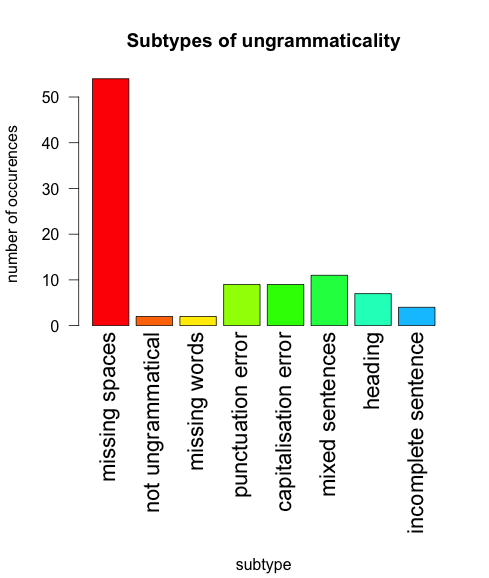
\includegraphics[scale=0.6]{subtypesWithText2.png}
\end{center}
\caption{\textbf{Subtypes of ungrammaticality in \textit{dev-1}.}}% A: nonword, B: not ungrammatical, C: missing words. D: punctuation error. E: capitalisation error. F: mixed sentences. G: heading. H: incomplete sentence (that was previously tagged as \texttt{other\_ungrammaticality})}
\label{subtypes}
\end{figure}

Perhaps the most noticeable result is the large portion of \textit{missing spaces} violations, meaning clauses that include tokens which aren't correct words. Almost all of these cases came from a missing space between two words forming tokens such as \texttt{reportsreaching} or \texttt{Wenchuancounty}. As there is such a large amount of this type, finding a reliable detection method for this subtype would significantly boost detection of ungrammaticality in general.

\section{Method}

The annotation, our work and the evaluation are done on sentence basis. As the text isn't split into sentences in the raw corpus, we use Stanford CoreNLP for that task. %TODO: cite CoreNLP

Being the biggest amount of cases of ungrammaticality, \textit{missing spaces} violations seem to have a straightforward solution which we call the \textbf{UnknownTokens} approach: Tagging a sentence as containing a \textit{missing spaces} ungrammaticality if there is a token that isn't a ``known'' token, i.e. one that doesn't exist in a list of known words. Obviously, this doesn't include words for named entities yet, so as a further condition they should also not be tagged as such by a Named Entity Recognizer.

The Stanford Named Entity Recognizer \citep{stanfordNER} is a widely used, state-of-the-art NER that comes with a model for the English language. After it was set up with the toolchain that is used to interact with the LQVCorpus XML, a list of known tokens was generated from the first 20\% of the AFE part of the gigaword corpus \citep{gigaword} and violations of the type \textit{Other ungrammatical form} in \textit{dev-2} (the second 20\% of the LQVCorpus) were annotated with the corresponding subtype.

In order to increase recall for NER, we assume that words that start with a capital letter and are only followed by lower case letters are known words / named entities. Finally, we automatically check whether an unseen token has a wikipedia entry, which further improves precision. We automatically label any tokens that are neither on our list of known tokens from GigaWord, nor tagged as a named entity as ``unknown''. 

\section{Evaluation}

We evaluate our experiments using the well-known metrics \textbf{P}recision, \textbf{R}ecall, \textbf{F}-Score and \textbf{A}ccuracy:

\begin{equation*}
	P = \frac{tp}{tp+fp} \quad R = \frac{tp}{tp+fn}
\end{equation*}
\begin{equation*}
	F = 2 * \frac{P * R}{P + R} \quad A = \frac{tp+tn}{tp+tn+fp+fn}
\end{equation*}

For experiment 1, we test how well our system works for detecting missing spaces. All sentences in \texttt{dev-2} that are correctly classified as \texttt{other ungrammatical form} with the subtype \texttt{missing spaces} are seen as true positives ($tp$), the ones it missed as false negatives($fn$). Sentences wrongly tagged as containing missing spaces are counted towards false positives($fp$) and finally, everything else is a true negative ($tn$).

In experiment 2, with the same data, we use the \textit{missing spaces} type as a measure for ungrammaticality and thus consider a sentence a true positive if our system detects a nonword and the sentence is tagged as ungrammatical in the corpus.

% \begin{table}

% \begin{center}
% \begin{tabular}{l|r|r}
% & Experiment 1 & Experiment 2 \\
% \hline
% Precision & 42.85\% & 57.14\% \\
% \hline
% Recall & 100.00\% & 53.33\% \\
% \hline
% Accuracy & 95.03\% & 92.54\%\\
% \hline
% F-Score & 59.99\% & 55.17\%\\
% \end{tabular}
% \end{center}
% \caption{Evaluation of \textbf{UnknownTokens}, experiments 1 and 2}
% \label{eval1}
% \end{table}

% \begin{table}

% \begin{center}
% \begin{tabular}{l|r|r}
% & Experiment 1a & Experiment 2a \\
% \hline
% Precision & 57.14\% & 71.42\% \\
% \hline
% Recall & 88.89\% & 25.64\% \\
% \hline
% Accuracy & 95.65\% & 79.50\%\\
% \hline
% F-Score & 69.56\% & 37.73\%\\
% \end{tabular}
% \end{center}
% \caption{Evaluation of \textbf{UnknownTokens}, experiments 1a and 2a}
% \label{eval2}
% \end{table}

\begin{table}

\begin{center}
\begin{tabular}{l|r|r|r|r}
& Precision & Recall & Accuracy & F-Score \\
\hline
Experiment 1 (missing spaces) & 42.85\% & 100.00\% & 95.03\% & 59.99\% \\
\hline %WARUM TODO SIND HIER DIE ACCURACIES IUNTERCSHIEDLICH
Experiment 1 (no missing spaces) & 96.05\% & 99.32\% & 95.65\% & 97.66\% \\
\hline
Experiment 1+wiki (missing spaces) & 78.04\% & 88.89\% & 98.14\% & 83.11\% \\ %80, 88.89, 98.14, 84.21
\hline
Experiment 1+wiki (no missing spaces) & 98.68\% & 99.34\% & 98.17\% & 99.01\% \\ %groß rausstellen
\hline
%Experiment 1a & 57.14\% & 88.89\% & 95.65\% & 69.56\% \\
%\hline
Baseline (missing spaces) & 0\% & 0\% & 94.40\% & 0\% \\ %tp & fp == 0
\hline
Baseline (no missing spaces) & 94.40\% & 100\% & 94.40\% & 97.12\% \\
%\hline
%Experiment 2 & 57.14\% & 53.55\% & 92.54\% & 55.17\% \\
%\hline
%Experiment 2a & 71.42\% & 25.64\% & 79.50\% & 37.73\% \\
\end{tabular}
\end{center}
\caption{Evaluation of \textbf{UnknownTokens}} %auf dev-1? dev-2?
\label{eval3}
\end{table}
\begin{table}

\begin{center}
\begin{tabular}{l|r}
& Experiment 1 (missing spaces/no missing spaces) \\
\hline
Micro-average precision & 92.77\% \\
\hline
Macro-average precision & 69.45\% \\
\hline
Micro-average recall & 98.72\% \\
\hline
Macro-average recall & 99.66\% \\
\hline
Micro-average F-score & 95.65\% \\
\hline
Macro-average F-score & 78.83\% \\
\end{tabular}
\end{center}
\caption{Macro- and micro-averages for \textbf{UnknownTokens}} %in große tabelle

%TODO Anzahl Instanzen Reinschreiben!! TODO DANGER!! sort-of done, BUT NOT REALLY

%TODO Fehlerfälle angucken und gucken, was noch machen

%tokens von originaldokumenten nehmen TODO

% rohdaten sind hier: summarization/data/tac/TAC_2011_Guided_Summarization_Task/GuidedSumm2011_test


%ToDO weka daten/ergebnisse Anne schicken, vorher! done

%TODO ein paar source-dokumente mit dependency-parser parsen

%TODO mapping schreiben (Stichwort: plagiarism detection)
% 10 ungrammatical (ohne unknown_tokens) parsen und satz "vorbereiten" (für mit manfred besprechen)
\label{eval3}
\end{table}


A evaluation lead to the results shown in Table~\ref{eval3}. The perhaps surprisingly high accuracy is due to the fact that the ``correct'' sentences outweigh the ungrammatical ones, leading to a high true negative count. This can also be seen in the baseline, which consists of tagging every word as not containing a \textit{missing spaces} violation.

In a second set of experiments (1a and 2a, also shown in Table~\ref{eval3}), we varied the settings of our previous experiments: In experiment 1a, we additionally annotated sentences of the violation type \texttt{incomplete sentence} with the subtype nonword, if applicable. In experiment 2a, we looked into how good the system could decide whether a sentence was either one of \texttt{incomplete sentence} or \textit{other ungrammatical form}, which lead to an increased precision, along with a severe decline in recall, because most incomplete sentences don't contain nonwords. It is to be expected that combining this approach with a seperate system for detection of cutoff sentences will lead to a much higher performance.

%eigene Todo:
% parser + arff

\section{Discussion}

When looking into the false positives, this result can be broken down to one main issue:

Clauses can contain multiple violations, such as \textit{other ungrammatical form} and \textit{incomplete sentence}. As only one of them was annotated, and the subtype was only added to clauses of the ungrammaticality type \textit{other ungrammatical form}, a large portion of the false positives isn't actually detected incorrectly, but rather not fully annotated. The fragment

\begin{quote}
	A spokesman for al-Aqsa Martyrs Brigades, armed wing \textbf{ofPalestinian}\\
	Fatah movement, denied on Monday the reports that \textbf{thetwo} suicide
\end{quote}

was annotated (correctly) as \textit{incomplete sentence}, but it is clear that the sentence also contains general ungrammaticality. As such, the system detected it as an unknown token and was punished for that decision.\todo{Adressed in exp 1a and 2a, rewrite}
\newpage
\bibliography{referenzen}
\bibliographystyle{apalike}

% UnknownTokens_source (in braces: for other class):

% FP: 3 {FN}
% FN: 4 {FP}
% TP: 70 {TN}
% TN: 1342 {TP}
% N: 1346 {P}
% P: 73 {N}

% Precision: 70/73 = 95.89% {1342/1346 = 99.70%}
% Recall: 70/(70+4) = 94.59% {1342/(1342+4) = 99.70%}
% F-Score: 2*((.9589*.9459)/(.9589+.9459)) = 95.24% {99.70%}

% weighted: 74 instances vs. 1345 non-instances -> 5.21%
% weighted precision: .9589*.0521 + .997*.9479 = 99.50%
% weighted recall: .9459*.0521 + .997*.9479 = 99.43%
% weighted F-Score: .9524*.0521 + .997*.9479 = 99.47

% micro-average precision: (70+1342)/(1346+73) 99.50%
% micro-average recall: (70+1342)/(70+1342+4+3) 99.50%
% micro-average F-score: 99.5%

% macro-average precision: 97.80%
% macro-average recall: 97.15%
% macro-average f-score: 97.47%


% UnknownTokens_general (in braces: for other class):

% FP: 30 {FN}
% FN: 3 {FP}
% TP: 71 {TN}
% TN: 1315 {TP}
% N: 1318 {P}
% P: 101 {N}

% precision 71/101 = 70.30% {1315/1318=99.77%}
% recall 71/(71+3) = 95.95% {1315/(1315+30) = 97.77%}
% f-score 2*70.3*95.95/(70.3+95.95) = 81.15% {98.76%}

% weighted: (see above)
% weighted precision: .703*.0521+.9977*.9479 = 98.23%
% weighted recall: .9595*.0521+.9777*.9479 = 97.68%
% weighted f-score: .8115*.0521+.9876*.9479 = 97.84%

% micro-average precision: (71+1315)/(101+1318) = 97.67%
% micro-average recall: (71+1315)/(71+1315+3+30) = 97.67%
% micro-average f-score: 97.67%

% macro-average precision: 85.04%
% macro-average recall: 96.86%
% macro-average f-score: 90.57%


% Baseline (in braces: for other class):

% FP: 0 {FN}
% FN: 74 {FP}
% TP: 0 {TN}
% TN: 1345 {TP}
% N: 1419 {P}
% P: 0 {N}

% Precision: 0% {1345/1419 = 94.79%}
% Recall: 0% {1345/(1345+0) = 100%}
% F-Score: 0% {97.33%}
 
% weighted: (see above)
% weighted precision: .9479*.9479 = 89.85%
% weighted recall: .9479*1 = 94.79%
% weighted f-score: 92.26%

% micro-average precision: 1345/1419 = 94.79
% micro-average recall: 1345/(1345+74) = 94.79
% micro-average f-score: 94.79%

% macro-average precision: 47.40%
% macro-average recall: 50%
% macro-average f-score: 48.67%



\end{document}